\section{Фотоэлектронный умножитель}\label{section:secMapmt}

Многоанодный фотоэлектронный умножитель (МА ФЭУ) H12700 фирмы Hamamatsu \cite{}, появившийся на рынке в 2013 г., подробно охарактеризован в работе \cite{}. Он обладает следующими достоинствами: большая доля площади поперечного сечения, приходящаяся на светочувствительные пиксели, квадратная форма, что позволяет перекрывать без потерь значительные площади (плотность упаковки 87\%), малое время прохождения однофотоэлектронного сигнала через динодную систему, малый разброс этого времени от события к событию, низкие перекрёстные помехи и низкая скорость счета тепловых электронов. Свойства данного прибора показаны в табл. \ref{tabl:MAPMT}, по большинству параметров он превосходит своего предшественника МА ФЭУ H8500 \cite{}. Наряду с перечисленными достоинствами, имеются некоторые особенности, не имеющие аналогов в традиционных ФЭУ и требующие особого внимания при реализации канала считывания. (отсюда прыгаем вниз на 20 строчек?)

\begin{table}[h]
\caption{Свойства МА ФЭУ H12700B-03.}
\label{tabl:MAPMT}
\begin{tabular}{ | p{0.25\linewidth} | p{0.25\linewidth} | p{0.25\linewidth} | p{0.25\linewidth} | }
	\hline
	Темновой счёт на канал, Гц & Темновой счёт на весь МА ФЭУ, кГц & Время нарастания сигнала, нс & Разброс времени развития электронной лавины, нс\\
	\hline
	$ \approx $ 10 & <1.0 & 0.64 & 0.28\\
	\hline
\end{tabular}
\end{table}

Данный МА ФЭУ имеет двухщелочной фотокатод. Спектральная чувствительность МА ФЭУ в версии H12700B-03, используемой в настоящей работе, соответствует конфигурации с входным стеклом, прозрачным в ультрафиолетовой области.

Коротковолновая граница спектра чувствительности $ \lambda_{min} $=185 нм, а максимум квантовой эффективности составляет 33\% и достигается при длине волны $ \lambda $=380 нм. Такие спектральные характеристики хорошо подходят для регистрации черенковского излучения, лежащего в ультрафиолетовой области. Среднеквадратичное отклонение коэффициентов усиления в каналах от среднего значения не превышает 16\% \cite{}. Разброс квантовой эффективности между пикселями составляет $ \pm $10\% \cite{}.

Имеются кривые  исследования \cite{}, показывающие, что радиационная стойкость прибора достаточна для использования в эксперименте CBM, также продемонстрирована работоспособность прибора в магнитном поле до 2.5 мТл \cite{}. Использование магнитных экранов и выбор оптимального расположения фотодетектора в пространстве делают этот МА ФЭУ пригодным для использования в эксперименте CBM. Отметим, что к этому прибору проявляют интерес и другие эксперименты, например, он рассматривается и для обновления LHCb \cite{}.

Обсудим особенности МА ФЭУ H12700B-03, важные для системы считывания. Размножение электронов в динодной системе происходит в одном и том же вакуумном объеме для всех каналов. Помещённая в единый вакуумный объём динодная система типа <<Metal Channel>>, см. \ref{fig:MetalChannel}, отличается тем, что она довольно компактна, едина для всех каналов и позволяет добиться отличных временных свойств. Электронные лавины, соответствующие разным каналам, отличаются местом прохождения через динодную систему. Имеют место такие эффекты как выбивание электронов из динодов фотонами, прошедшими сквозь фотокатод, и отклонение электронов от идеальной траектории за счет разброса энергий. Последняя особенность приводит к попаданию электронов на последующие стадии динодной системы, минуя предыдущие, и перетеканию всей или части электронной лавины в соседний канал. Перетекание части лавины в соседний канал имеет место в более чем 25\% случаев при равномерном освещении всего фотокатода. Величина перетекающего заряда составляет от 3\% до 7\% в зависимости от взаимного расположения пикселей \cite{}. Вероятность того, что лавина от фотоэлектрона полностью разовьётся в соседнем канале зависит от взаимного расположения каналов и составляет при равномерном освещении от 0.1\% до 2\%. В классическом ФЭУ такие эффекты отсутствуют из-за наличия развитой системы фокусировки и такой конструкции динодной системы, что диноды имеют большую площадь и последующие стадии полностью экранируются предыдущими.

\begin{figure}
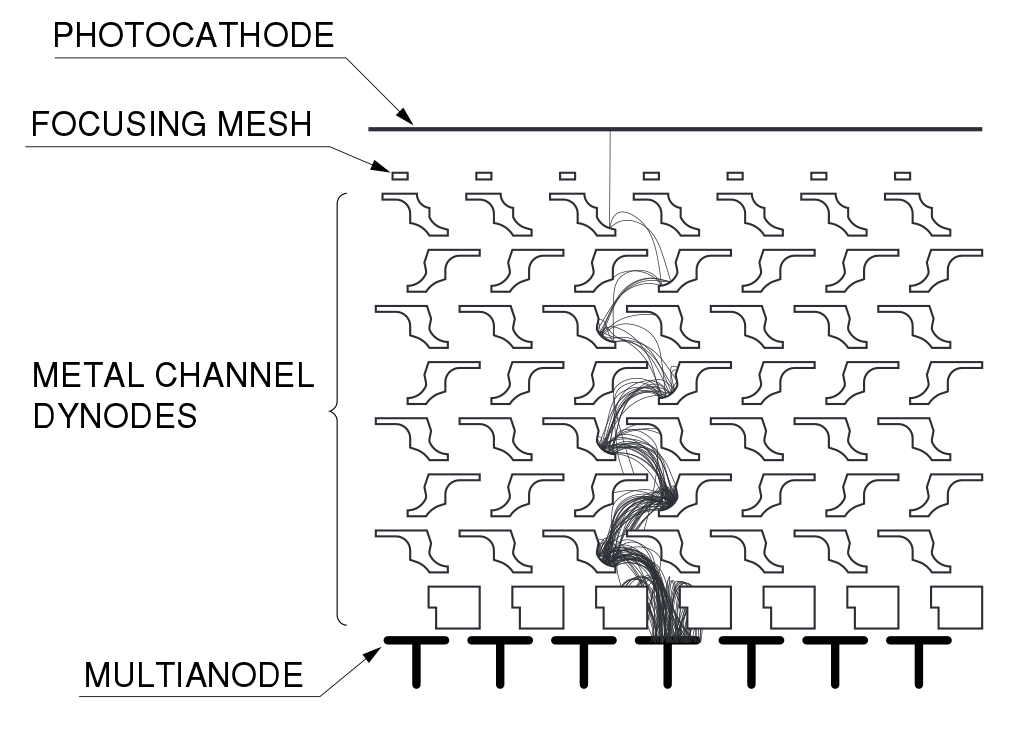
\includegraphics[width=1.0\textwidth]{pictures/2_Metal_channel.png}
\caption{Схема динодной системы типа <<Metal Channel>>.}
\label{fig:MetalChannel}
\end{figure}

Описанные особенности приводят к формированию в одноэлектронном спектре низкоамплитудной части, сливающейся с шумами и отделенной от основного пика довольно глубокой ложбинкой, см рис. \ref{fig:SPEspectrum}. Проявления этого эффекта в наших измерениях обсуждаются в секции \ref{}.

\begin{figure}
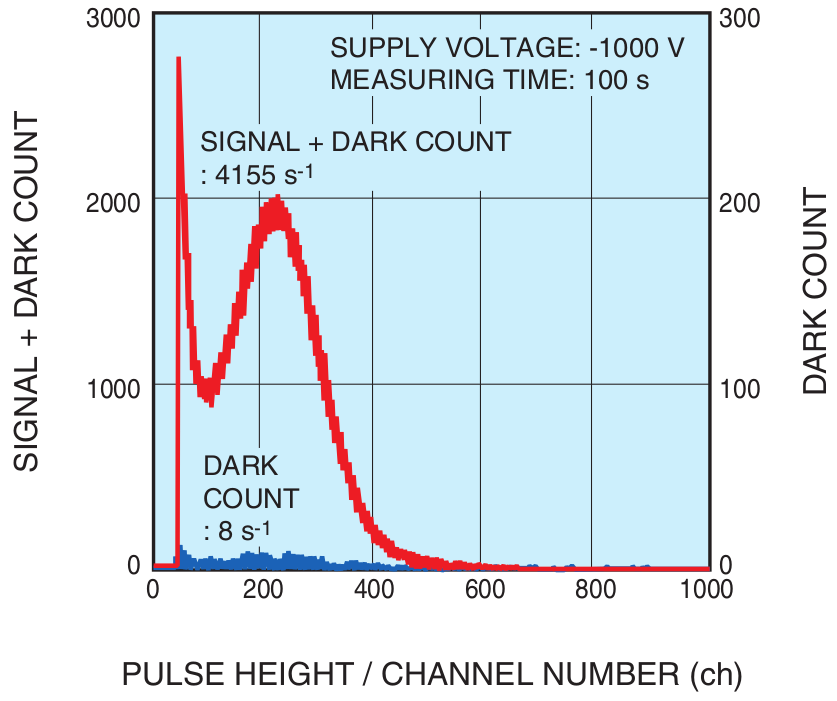
\includegraphics[width=1.0\textwidth]{pictures/3_Typical_spectrum_from_H12700.png}
\caption{Типичный одноэлектронный спектр.}
\label{fig:SPEspectrum}
\end{figure}
